\chapter{Diseño}
\label{chap:diseño}

\section{Arquitectura de la aplicación}
Para representar la arquitectura de la aplicación, se ha recurrido a diagramas C4 \cite{brownc4model}, que permiten describir el sistema a diferentes niveles de abstracción, desde una visión general hasta los detalles de implementación. A continuación, se detallarán los tres primeros niveles de este modelo, llegando hasta el diagrama de componentes.

\subsection{Diagrama de contexto (Nivel 1)}
El nivel del diagrama de contexto proporciona una visión general del sistema, mostrnado las interacciones entre el sistema, los usuarios y otros sistemas externos.

Los principales actores identificados en el diagrama de contexto son:
\begin{itemize}
    \item \textbf{Usuario:} Actor humano que interactúa con la aplicación para gestionar su trabajo, colaborar en proyectos y comunicarse con otros usuarios y agentes.
    \item \textbf{Sistema}: Plataforma que proporciona las funcionalidades anteriormente descritas.
    \item \textbf{Proveedor de autenticación:} Servicio externo responsable de gestionar la autenticación de los usuarios (ej. Google).
    \item \textbf{Proveedores de \ac{IA}:} Servicios externos que ofrecen modelos \ac{IA} para procesar prompts del módulo de agentes (ej. OpenAI, Anthropic).
\end{itemize}    

\begin{figure}[ht]
    \centering
    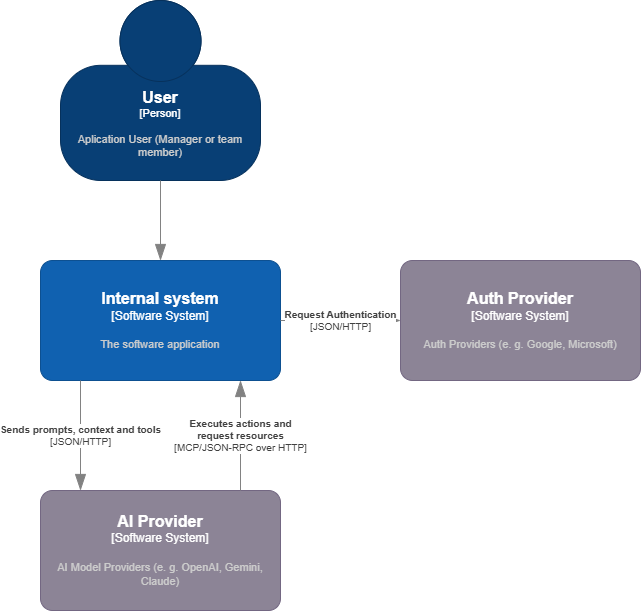
\includegraphics[width=0.8\textwidth]{images/content/Diseño/level1.png}
    \caption{Diagrama de contexto de la aplicación}
    \label{fig:diagrama_contexto}
\end{figure}

\subsection{Diagrama de contenedores (Nivel 2)}
Descendiendo al siguiente nivel de detalle, el diagrama de contenedores muestra las unidades de ejecución del sistema (aplicaciones, servicios, bases de datos), así como las responsabilidades de cada una y cómo se comunican entre sí.

Los contenedores identificados en el diagrama son:
\begin{itemize}
  \item \textbf{\emph{Frontend}:} Aplicación web \ac{SPA} ejecutada en el navegador del usuario, actúa como interfaz gráfica para interactuar con el sistema. Su responsabilidad es la composición visual de la interfaz, delegando la lógica de negocio al \emph{backend} a través de llamadas a la API REST.
  \item \textbf{\emph{Backend}:} Forma el núcleo del sistema, implementando la lógica de negocio, además de orquestar la comunicación entre diferentes servicios y gestionar la persistencia de datos. Expone una API REST para que el \emph{frontend} pueda interactuar con él, y también se encarga de comunicarse con los proveedores externos (autenticación y \ac{IA}).
  \item \textbf{Bases de datos:} Cumpliendo de forma estricta con los principios de \ac{DDD}, cada módulo o \emph{Bounded Context} tiene su propia base de datos, garantizando la independencia y autonomía de cada uno. Esto permite que cada módulo evolucione de forma aislada, sin afectar a los demás, y facilita la implementación de diferentes tecnologías de almacenamiento si fuera necesario. Esta separación anticipa una separación física futura en microservicios que se analiza más adelante al entrar al detalle del \emph{backend}.
  \item \textbf{Almacenamiento de objetos:} Contenedor de infraestructura dedicado a almacenar archivos y recursos estáticos, como imágenes, documentos o cualquier otro tipo de archivo que deba ser accesible desde la aplicación. Se utiliza principalmente para almacenar los archivos adjuntos a los elementos de trabajo. Este almacenamiento recibe lecturas y escrituras directamente desde el \emph{frontend}, aliviando así la carga del \emph{backend} y mejorando la escalabilidad del sistema, para mantener la seguridad, el acceso a este almacenamiento se gestiona mediante URLs firmadas que permiten un acceso temporal y controlado a los recursos almacenados.
  \item \textbf{Servidor de logs:} Contenedor de infraestructura encargado de centralizar y gestionar los logs generados por el sistema. Este contenedor recolecta, indexa y almacena los logs, trazas de ejecución y métricas de rendimiento producidos por la aplicación. Su uso permite monitorizar el estado del sistema, detectar errores y analizar el comportamiento de la aplicación, por lo que es una herramienta añadida únicamente para mejorar la mantenibilidad del sistema.
\end{itemize}

\begin{figure}[ht]
    \centering
    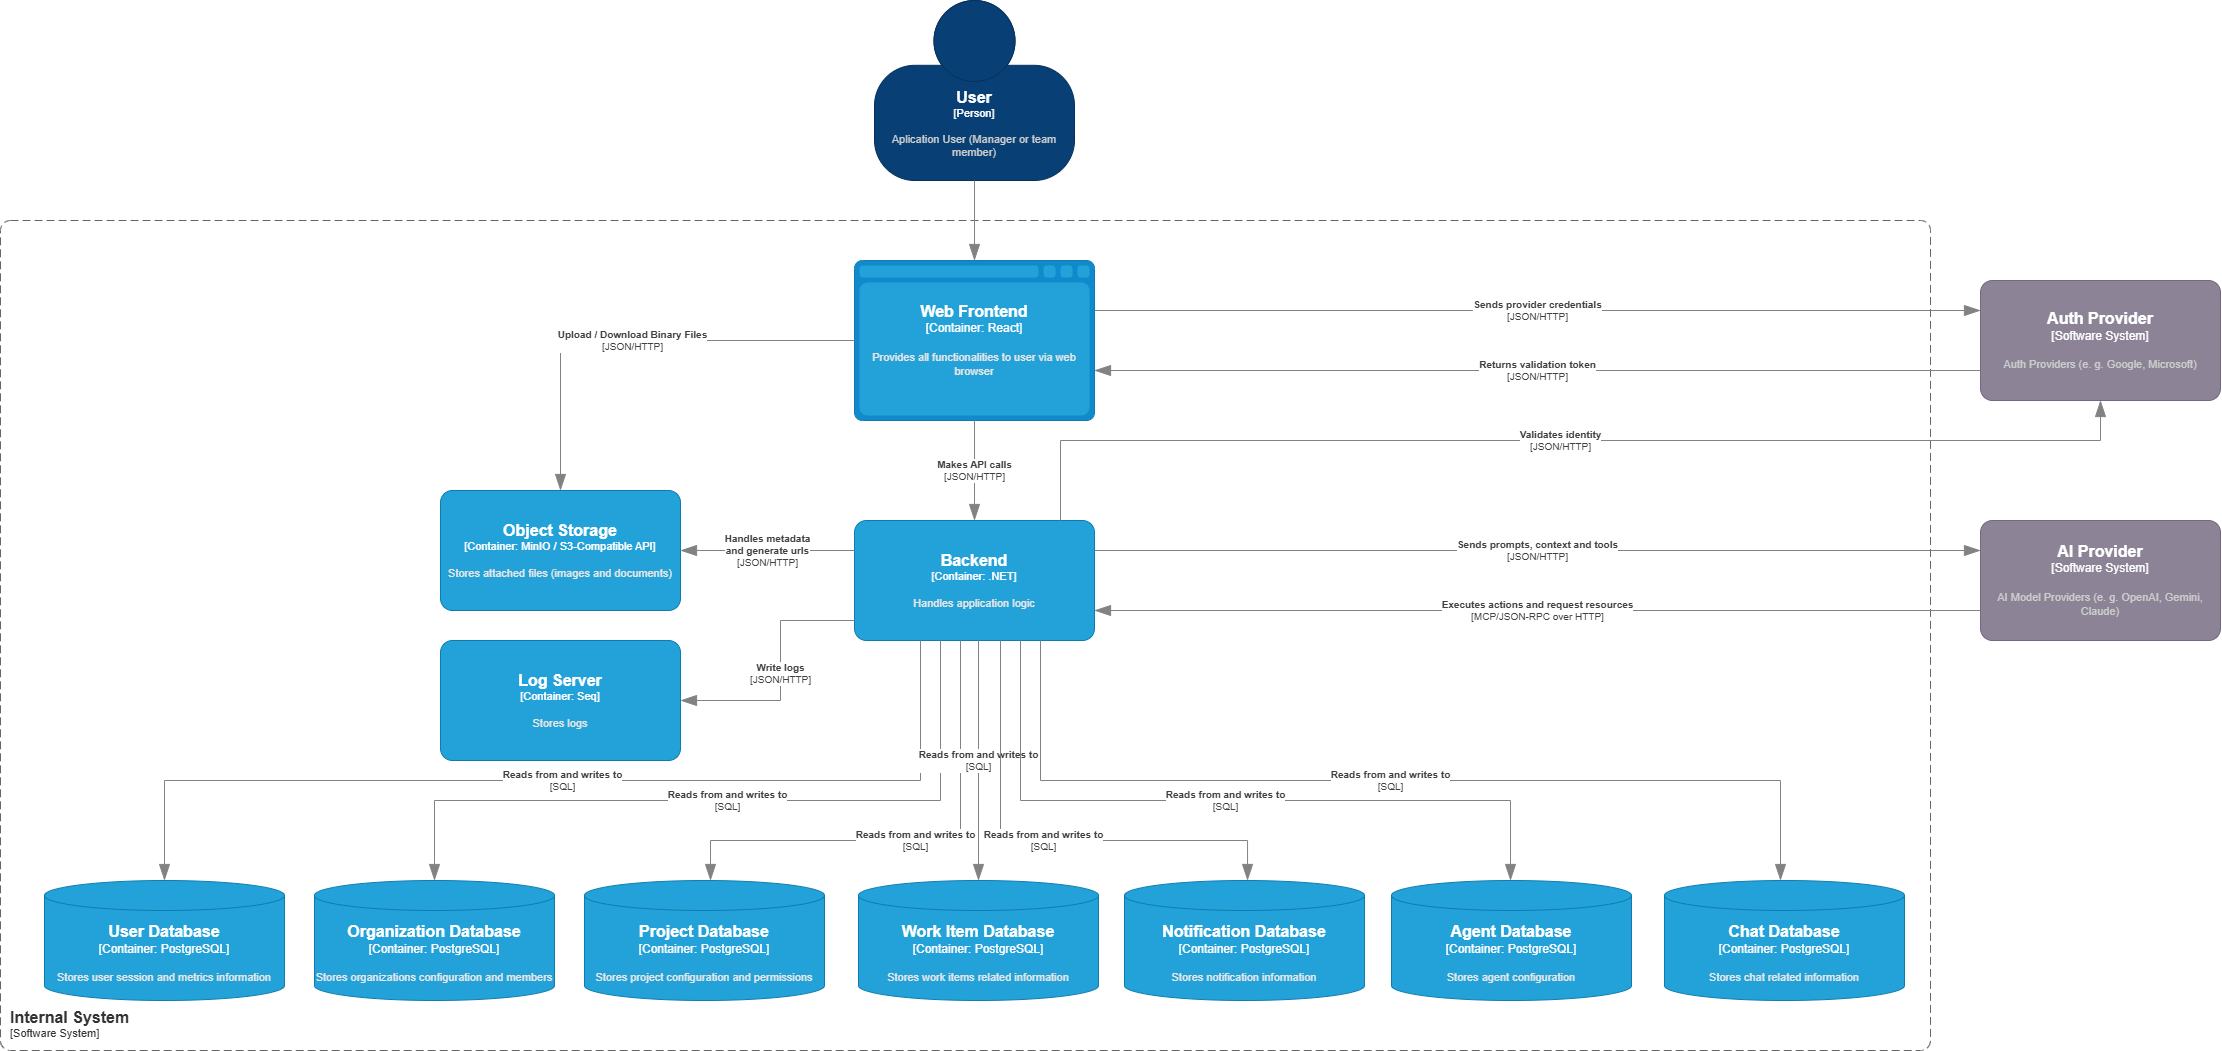
\includegraphics[width=0.8\textwidth]{images/content/Diseño/level2.png}
    \caption{Diagrama de contenedores de la aplicación}
    \label{fig:diagrama_contenedores}
\end{figure}

\subsection{Diagrama de componentes (Nivel 3)}
Para diagramar a nivel de componentes, haremos un desglose en cada uno de los contenedores principales identificados en el nivel anterior.

\subsubsection{\emph{Backend}}
En este nivel de detalle del \emph{backend}, observamos ya una clara separación en módulos que se corresponden con los \emph{Bounded Contexts} identificados en el análisis del dominio. La arquitectura adoptada para el sistema es la de un \emph{monolito modular}. A diferencia de un monolito tradicional ,donde la falta de fronteras estrictas tiende a generar un alto acoplamiento y dificulta el mantenimiento, y de una arquitectura pura de microservicios, que introduce una alta sobrecarga operativa y complejidad de red desde el primer día, el monolito modular ofrece un equilibrio pragmático \cite{newman2019monolith}. Cada módulo encapsula su propia lógica de negocio y funciona de forma autónoma, lo que asegura un bajo acoplamiento y facilita enormemente una futura separación física en microservicios si las necesidades de escalabilidad del proyecto lo llegasen a requerir.

Para garantizar esta autonomía, la comunicación entre los distintos módulos se realiza a través de interfaces bien definidas mediante eventos y colas de mensajería asíncrona \cite{hohpe2004enterprise}. Esta independencia maximiza la escalabilidad lógica de cada contexto, pero introduce complejidad en la gestión de los datos. Al prescindir de la transaccionalidad global e inmediata de las bases de datos centralizadas, el diseño del sistema debe afrontar las disyuntivas descritas por el Teorema CAP \cite{gilbert2002brewer}. En este escenario, la aplicación prioriza la disponibilidad y el aislamiento de los módulos, asumiendo un modelo de \emph{consistencia eventual}. Para manejar eficazmente esta separación entre la emisión de eventos y la actualización de los estados, el sistema se apoya en el patrón \ac{CQRS} \cite{fowler2007cqrs}, optimizando de forma independiente los flujos de lectura y escritura.

El detalle técnico sobre cómo se orquesta esta arquitectura orientada a eventos de la comunicación asíncrona entre módulos se detallará más adelante en este mismo capítulo, donde se ilustrará el proceso apoyándose en un diagrama de secuencia explicativo.

Revisando ahora los componentes que encontramos en este diagrama, observamos:

\begin{itemize}
  \item \textbf{Módulos:} Un componente referente a cada uno de los módulos identificados, que funcionan de forma independiente.
  \item \textbf{API \emph{Host}:} Es el punto de entrada de la aplicación, se encarga de levantar el servidor web, gestionar las rutas y configurar cada uno de los módulos para que estén disponibles a través de la API REST. 
  \item \textbf{Bus de eventos:} Componente central que facilita la comunicación asíncrona entre los módulos, permitiendo que cada uno emita eventos sin necesidad de conocer los consumidores de dichos eventos.
  \item \textbf{\emph{Background workers}:} Componentes encargados de procesar tareas en segundo plano, como la sincronización de datos entre módulos u otros procesos que no requieren una respuesta inmediata al usuario.
  \item \textbf{\emph{Building blocks}:} Componentes comunes que pueden ser utilizados por varios módulos,  cómo abstracciones, funcionalidades transversales para realizar llamadas, gestionar conexiones con las bases de datos, publicación y suscripción de eventos, etc.
\end{itemize}

\begin{figure}[ht]
    \centering
    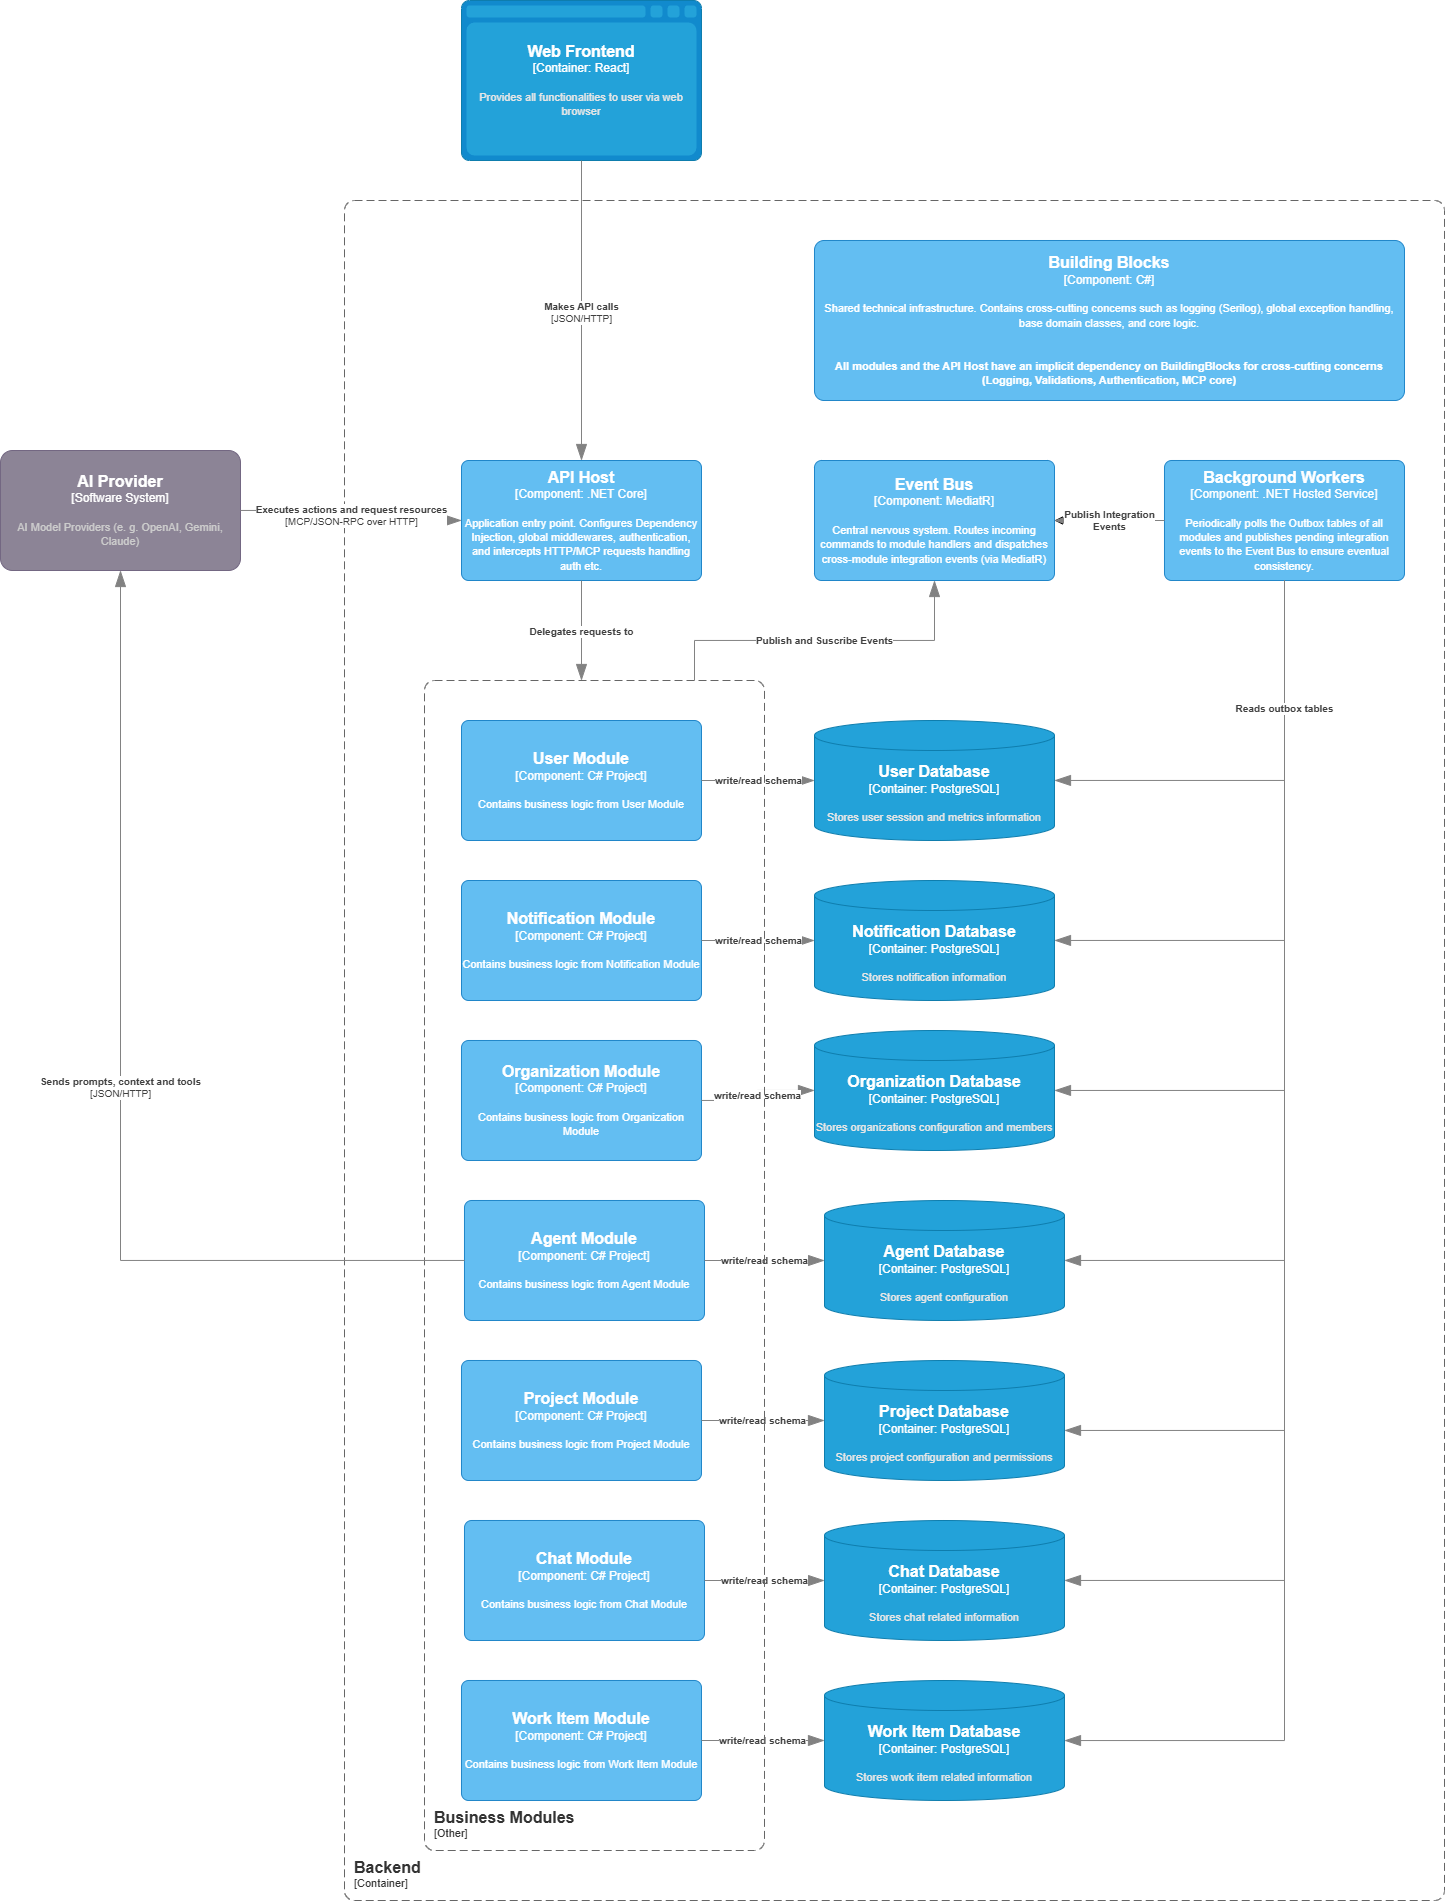
\includegraphics[width=0.8\textwidth]{images/content/Diseño/level3-backend.png}
    \caption{Diagrama de componentes del \emph{backend}}
    \label{fig:diagrama_componentes_backend}
\end{figure}

\subsubsection{\emph{Backend} (dentro de un módulo)}
Entrando en el detalle de cada módulo, la arquitectura interna sigue los preceptos de la \emph{Clean Architecture} \cite{martin2017clean}, separando claramente las responsabilidades en capas concéntricas. 
En el núcleo se encuentran las entidades de dominio, que encapsulan la lógica de negocio pura y se mantienen independientes de cualquier tecnología o \emph{framework}. 
Alrededor de estas entidades, en la capa de aplicación, se ubican los casos de uso, encargados de orquestar la lógica de negocio y coordinar las interacciones para cumplir con los requisitos funcionales.

La capa de infraestructura se ha estructurado adoptando la topología de la Arquitectura Hexagonal (también conocida como patrón de Puertos y Adaptadores) propuesta por Cockburn \cite{cockburn2005hexagonal}. Con el añadido de que, esta capa de infraestructura se divide en dos: la \emph{Driving Infrastructure}, que recibe las solicitudes entrantes, las traduce y las dirige hacia los casos de uso; y la \emph{Driven Infrastructure} que se encarga de implementar las interfaces definidas por el dominio para interactuar con servicios externos, tales como bases de datos o APIs de terceros.

Es importante destacar que toda esta estructura se vertebra en torno al Principio de Inversión de Dependencias \cite{martin1996dependency}. La aplicación de este principio asegura que las dependencias a nivel de código fuente apunten hacia el centro del sistema, haciendo que el núcleo de la aplicación sea completamente independiente de las implementaciones tecnológicas concretas de las capas externas.

Además de estos componentes esenciales, cada módulo también incluye un componente de integración, que expone los eventos de integración que el módulo emite para que otros módulos puedan suscribirse a ellos.

\begin{figure}[ht]
    \centering
    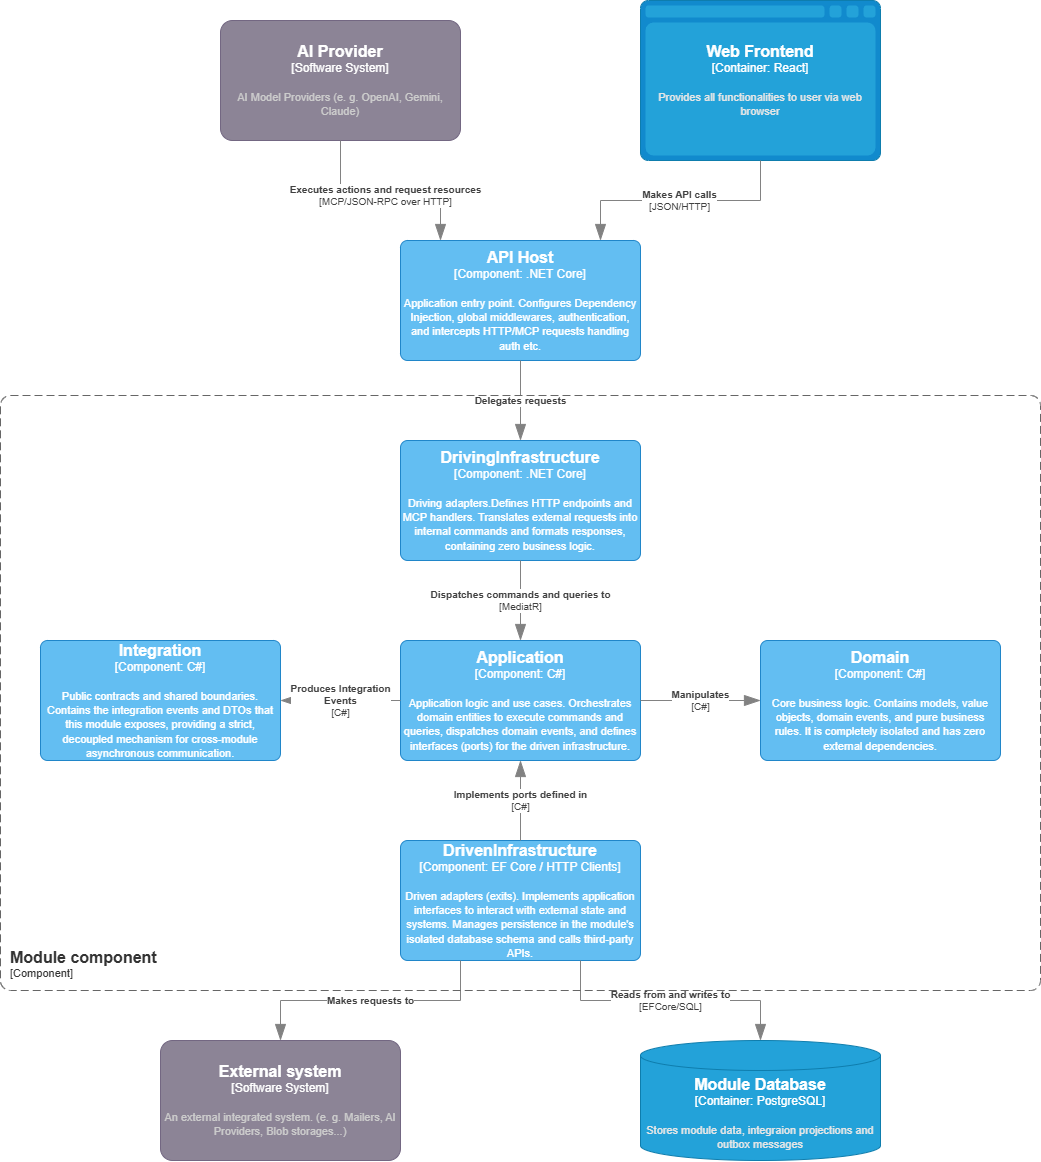
\includegraphics[width=0.8\textwidth]{images/content/Diseño/level3-module.png}
    \caption{Diagrama de componentes dentro de un módulo}
    \label{fig:diagrama_componentes_modulo}
\end{figure}

\subsubsection{\emph{Frontend}}
El \emph{frontend} de la plataforma se ha desarrollado como una aplicación web \ac{SPA} utilizando React, lo que permite ofrecer una experiencia de usuario fluida y sin recargas de página. La arquitectura del cliente se aleja de los enfoques clásicos basados en el patrón \ac{MVC}, para adoptar una arquitectura orientada a componentes que se alinea de forma natural con el ecosistema de React. Con el objetivo de mantener una alta cohesión y respetar las fronteras de los \emph{Bounded Contexts} definidos en el dominio, se ha optado por estructurar la aplicación mediante \emph{Vertical Slices} \cite{bogard2018vertical}, priorizando el pragmatismo y la agrupación por funcionalidades en lugar de por capas técnicas.

Para lograr una correcta separación de responsabilidades dentro de cada módulo, la aplicación se estructura internamente en tres capas principales:
\begin{itemize}
    \item \textbf{Capa de presentación:} Compuesta por los componentes visuales que conforman la interfaz de usuario. Utiliza de forma intensiva la metodología de Diseño Atómico (\emph{Atomic Design}) \cite{frost2016atomic} para garantizar la reutilización y la consistencia visual en toda la aplicación. A nivel organizativo, se divide en tres bloques: utilidades y componentes compartidos (\emph{shared}) que pueden ser consumidos por cualquier módulo; componentes específicos de dominio encapsulados en su respectivo módulo; y el componente \emph{Root Composition}, encargado del enrutamiento global y la composición final de la interfaz.
    \item \textbf{Capa de proveedores:} Contiene los proveedores de la API de Contexto (\emph{Context API}) de React que gestionan el estado global de la aplicación. Esta capa aísla y expone funcionalidades transversales críticas, tales como la autenticación, la gestión de sesiones de usuario y la internacionalización de la aplicación.
    \item \textbf{Capa de datos:} Encargada de abstraer y gestionar toda la comunicación asíncrona con el \emph{backend} mediante llamadas a la \ac{API} REST. Está formada por tres elementos principales: el cliente \ac{HTTP} base; el cliente \ac{API}, que actúa como un patrón \emph{Facade} \cite{gamma1994design} exponiendo métodos tipados y específicos para cada uno de los \emph{endpoints}; y finalmente el componente de \emph{queries}, que utiliza la biblioteca React Query \cite{tanstackquery} para optimizar el ciclo de vida de las peticiones, gestionando de forma eficiente el estado asíncrono, la caché de datos y la invalidación de la misma.
\end{itemize}